\documentclass{article}

% Language setting
% Replace `english' with e.g. `spanish' to change the document language
\usepackage[english]{babel}

% Set page size and margins
% Replace `letterpaper' with `a4paper' for UK/EU standard size
\usepackage[a4paper,top=2.3cm,bottom=3cm,left=3cm,right=3cm,marginparwidth=1.75cm]{geometry}

% Useful packages
\usepackage{amsmath}
\usepackage{graphicx}
\usepackage{appendix}
\usepackage[colorlinks=true, allcolors=blue]{hyperref}

\title{EES mini Project}
\author{Xiaoning Nie. (cshb26)}

\begin{document}
\maketitle

\


\section{Introduction}

\subsection{Description of the project}

In this project, the daily temperature data from 1901 to 2019 is provided to predict the average daily temperature in 2020.

There are many ways to complete this project, and here I choose to use \verb|prophet|, an open source Python package from Facebook, which is a time series forecasting package that helps us to tackle time-related problems easily.

\

\subsection{Description of the dataset}

By the analysis of the dataset we can see that it has a total of 43,464 samples, 8 features per sample and no missing values, as shown below in Figure 1.

\begin{figure}[hp]
\centering
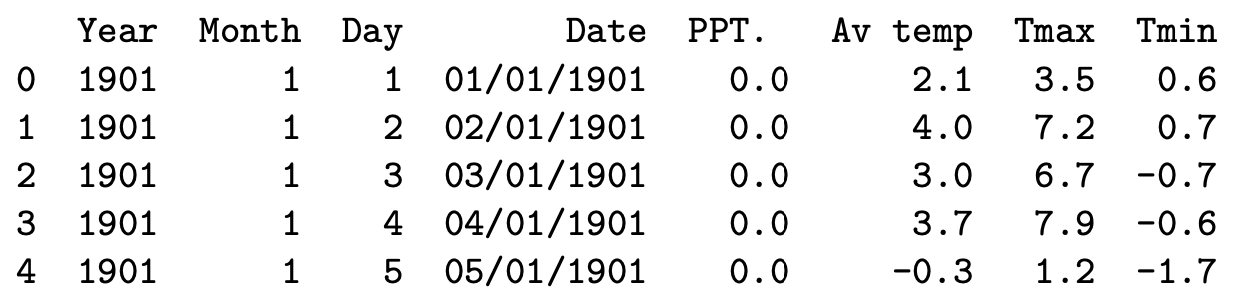
\includegraphics[width=12cm]{datadesc.png} %[图片大小]{图片路径}
\caption{First 5 samples in the dataset} %图片标题
\end{figure}

Where, the eight features represent:

\begin{itemize}
\item \verb|Year|, \verb|Month|, \verb|Day| and \verb|Date| describe the specific date of the temperature data;
\item \verb|PPT. | describes the daily rainfall;
\item \verb|Tmax| and \verb|Tmin| describe the daily maximum and minimum temperature;
\item \verb|Av temp| describes the daily average temperature, which is also the target.
\end{itemize}

\newpage

\section{Process \& Results}

\subsection{Data preprocessing}

According to the question, we need to predict the daily average temperature in 2020, so features \verb|Date|, \verb|Tmax| and \verb|Tmin| from previous years are not important to us, thus, they are discarded.

The relationship between daily rainfall and average daily temperature over the first 10 years is shown in Figure 2, from what we can see that there is no relationship between them, so the feature \verb|PPT.| is deleted directly.

\begin{figure}[htbp]
\centering
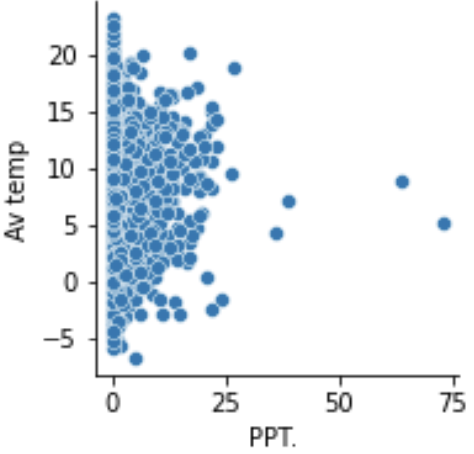
\includegraphics[width=5cm]{rela.png} %[图片大小]{图片路径}
\caption{Relationship between daily rainfall and average daily temperature} %图片标题
\end{figure}


\subsection{Prediction \& results}

At the end of preprocessing, the forecast begins. In this project, forecast is made using the Prophet model from the prophet package. Figure 3 is the visualisation of all the average daily temperature data from 1901 to 2020.

\begin{figure}[htbp]
\centering
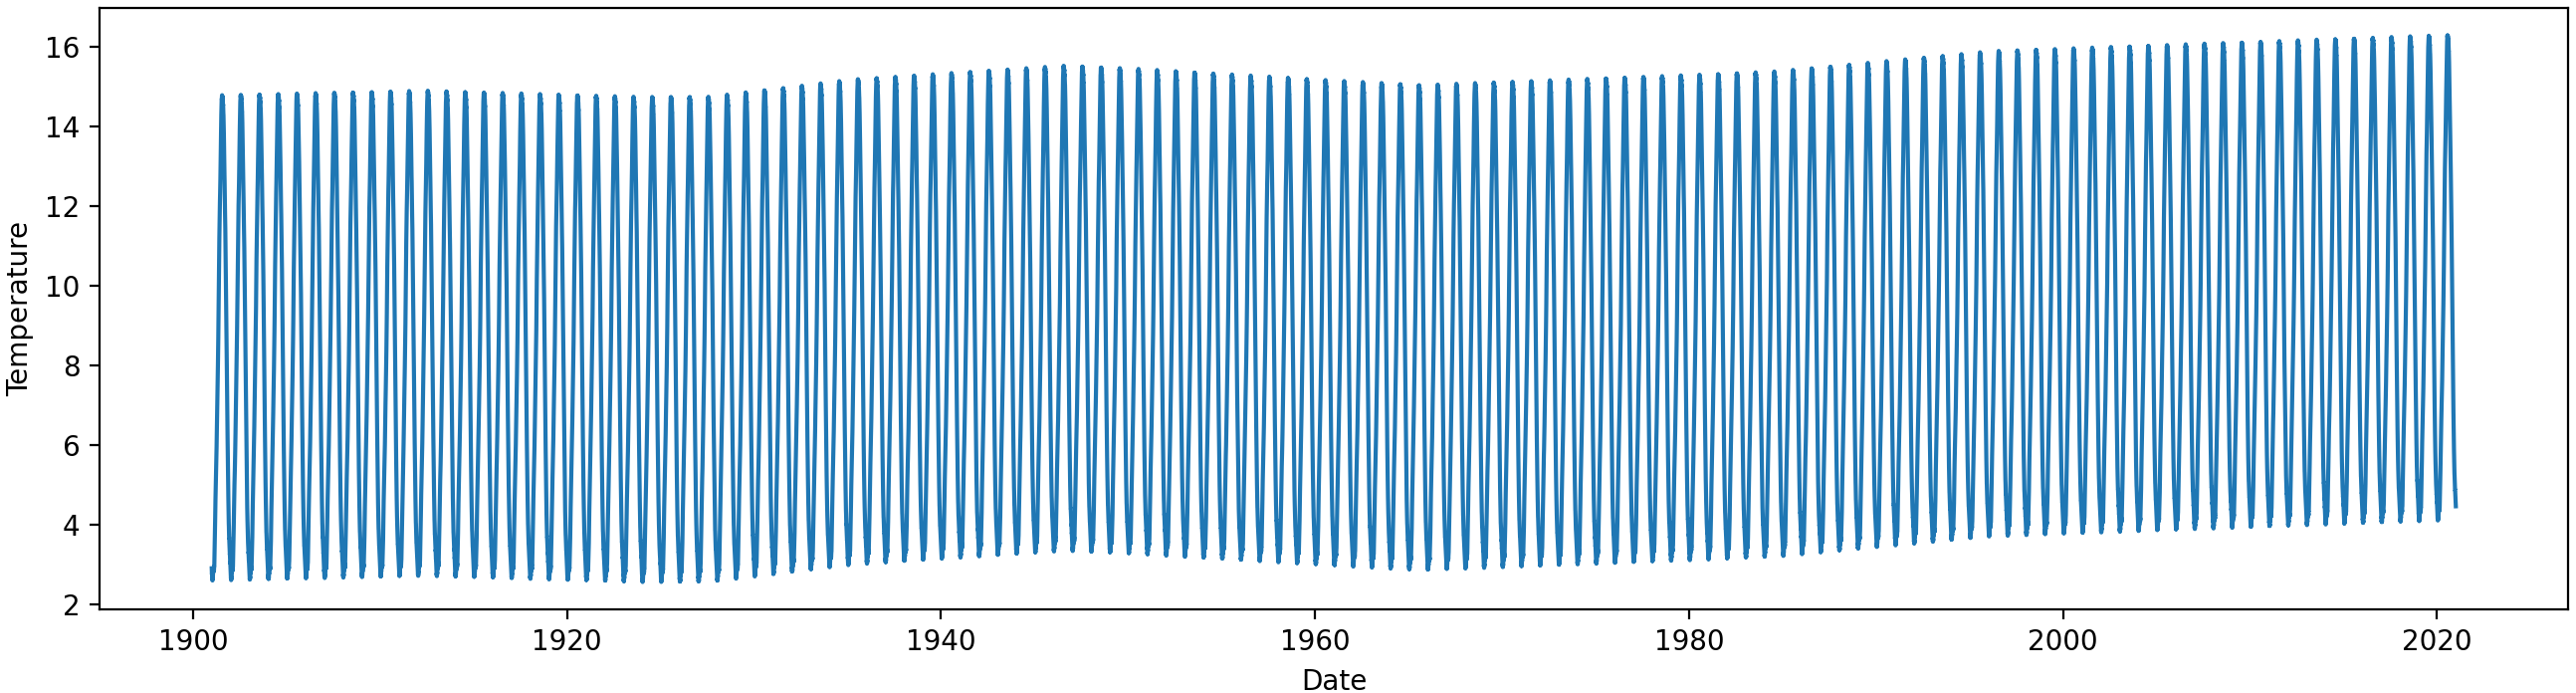
\includegraphics[width=13cm]{wholeyears.png} %[图片大小]{图片路径}
\caption{All temperature data from 1901 to 2020} %图片标题
\end{figure}

The average daily temperature for 2020 required in this project is shown in Figure 4.
\begin{figure}[htbp]
\centering
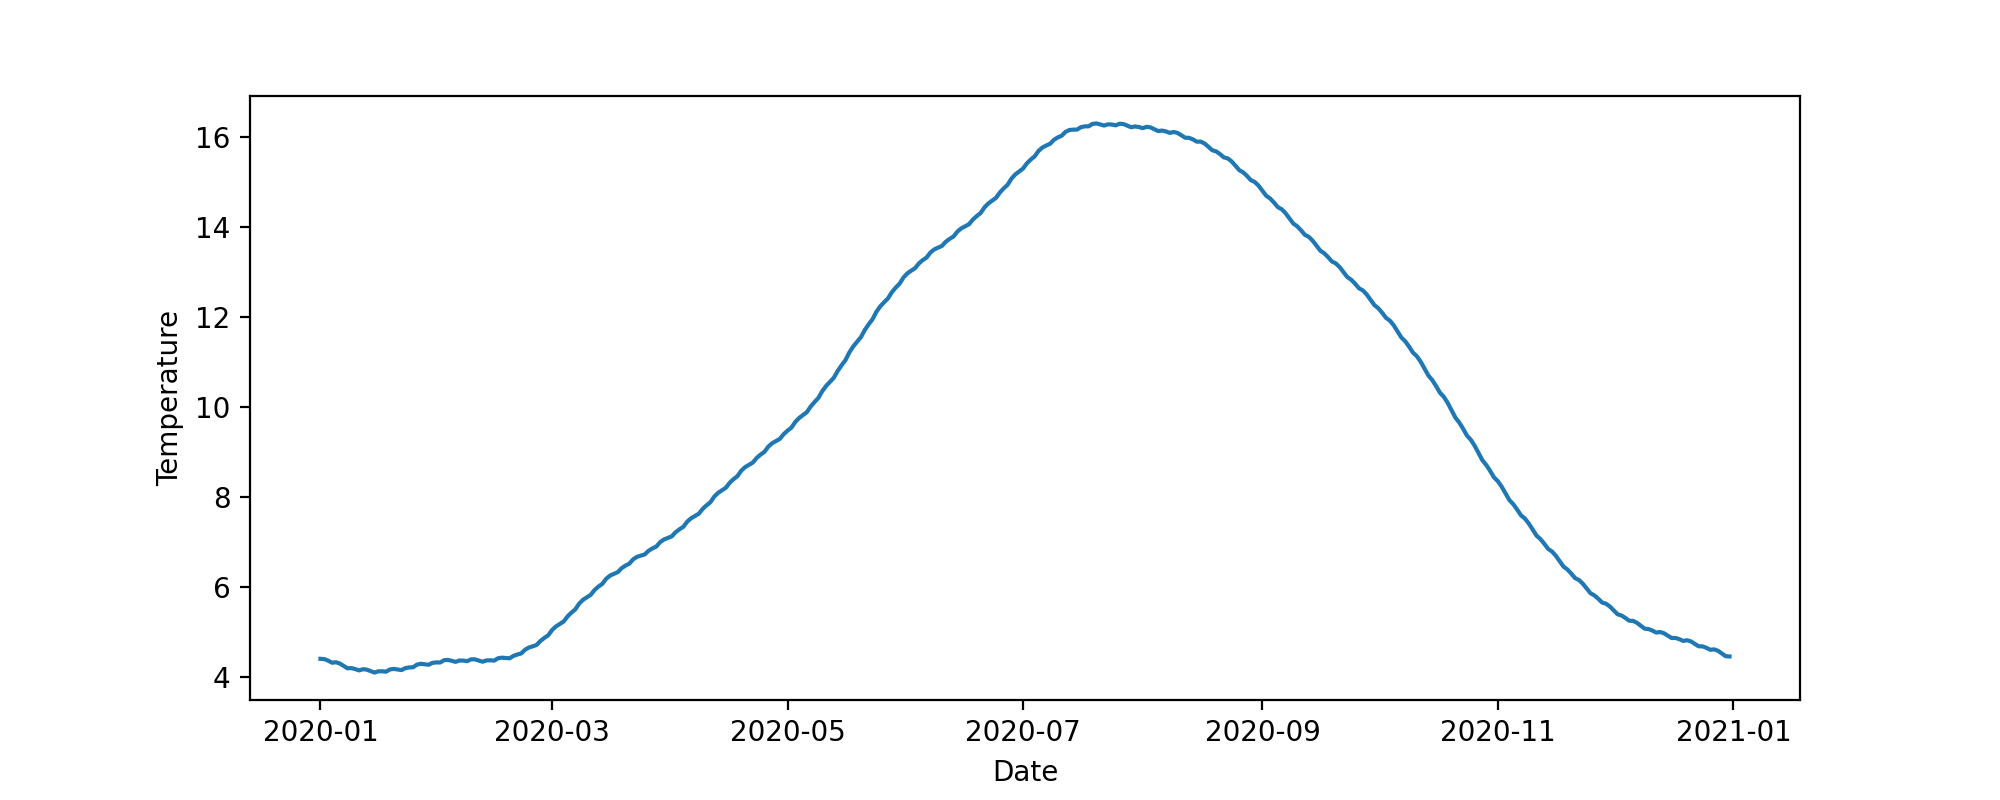
\includegraphics[width=13cm]{year2020.png} %[图片大小]{图片路径}
\caption{Predicted average daily temperature of 2020} %图片标题
\end{figure}


Meanwhile, from Figure 3 we can see that there is an increasing trend in the average annual temperatures from 1901 to 2020, so the average annual temperatures are plotted separately, as shown in Figure 5. From the graph we can easily see that the average annual temperatures have increased by 1.5 degrees centigrade over the past 120 years, which reflects the current global warming problem.

\begin{figure}[htbp]
\centering
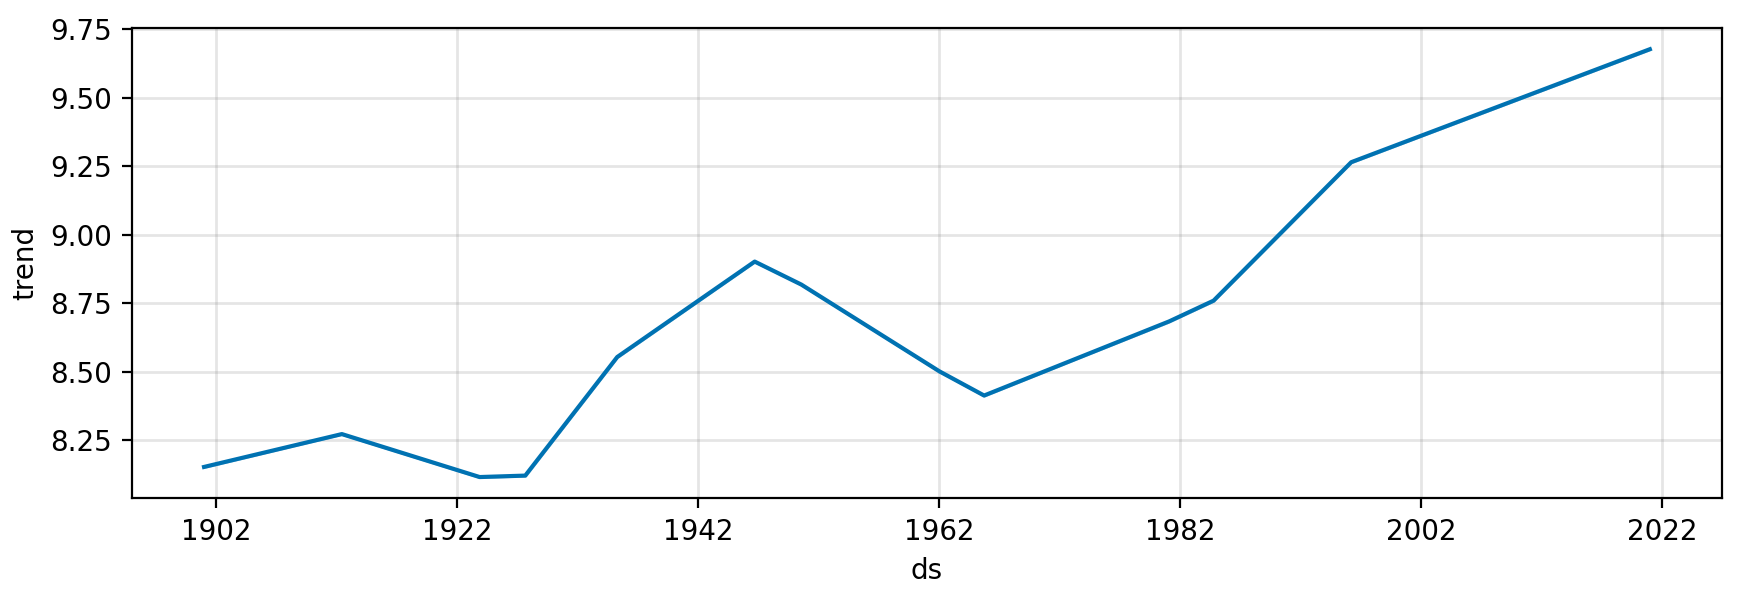
\includegraphics[width=15cm]{trend.png} %[图片大小]{图片路径}
\caption{The trend of average annual temperatures} %图片标题
\end{figure}


\subsection{Error analysis}

When I perform the error analysis on the forecasting data, we can see that the RMSE of the prediction is maintained at a low level as shown in Figure 6, which is acceptable in this project.

\begin{figure}[h]
\centering
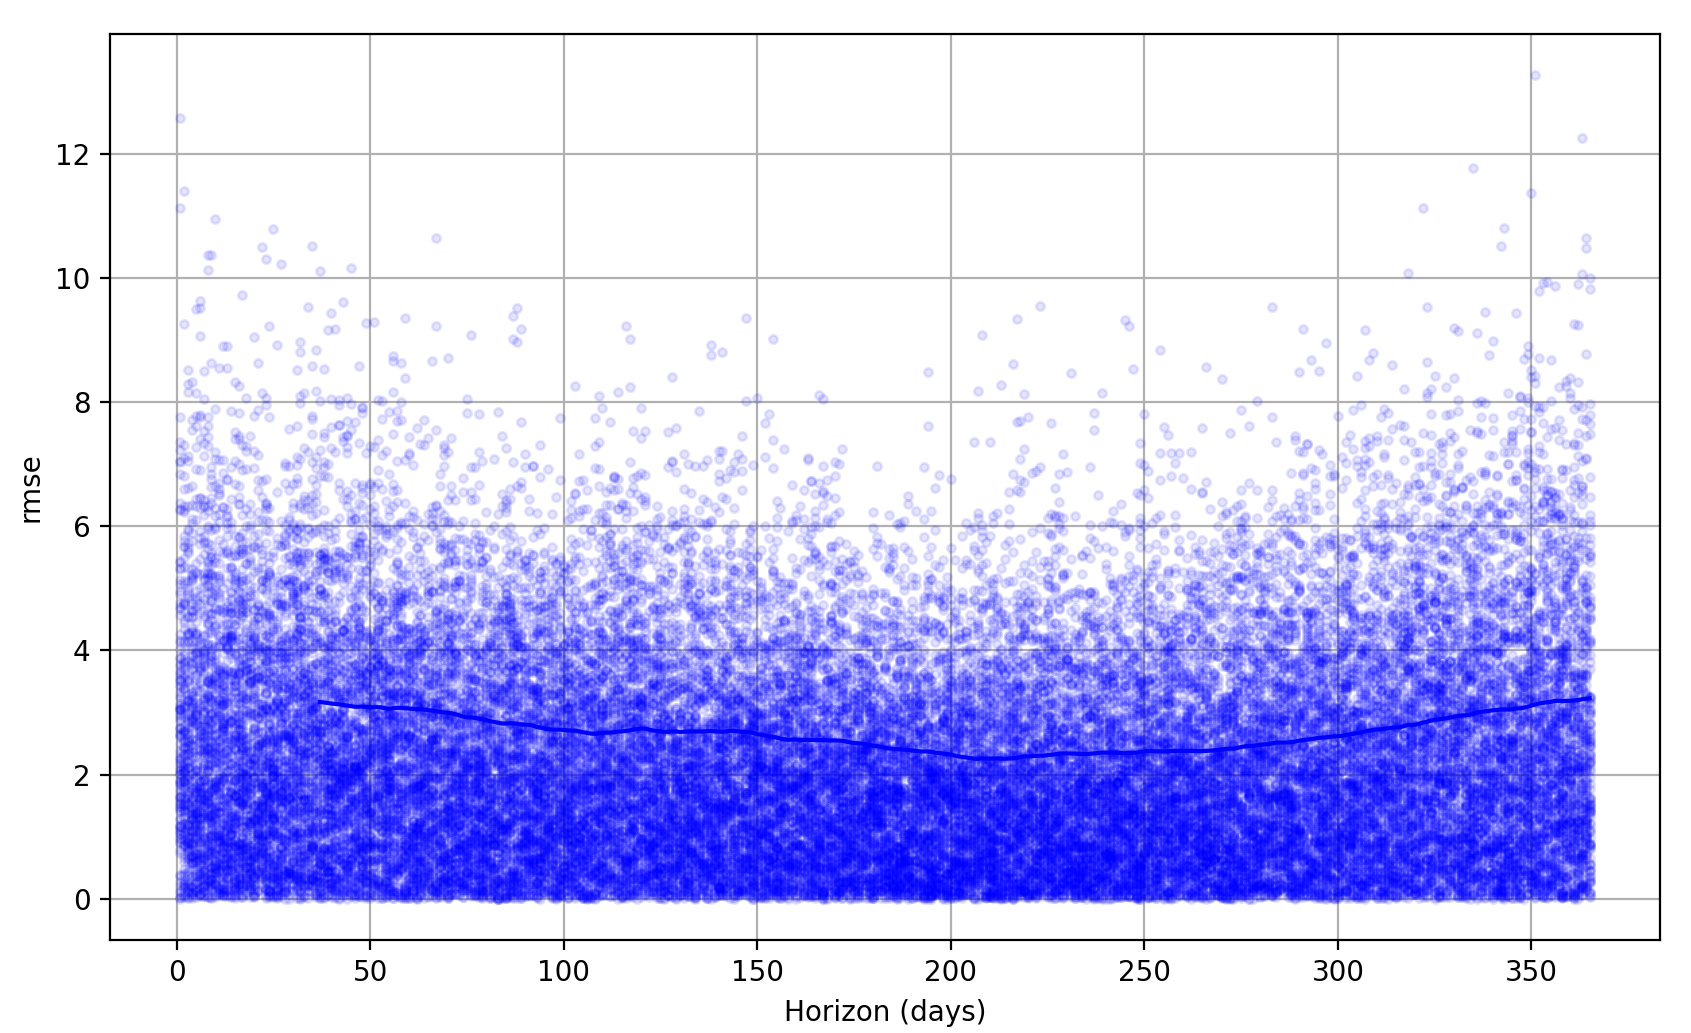
\includegraphics[width=12cm]{rmse.png} %[图片大小]{图片路径}
\caption{RMSE of the prediction} %图片标题
\end{figure}



\newpage


\section{Discussion}

\subsection{Reasons of choosing prophet}

Prophet is an open source time series data prediction tool developed by Facebook, which combines time series decomposition and machine learning. Its powerful performance can solve most actual scenarios of the time series prediction with high efficiency.

Prophet has several points that make me choose to use it for data prediction:

1. It does not require much feature engineering to obtain the future trends and data.

2. It allows almost fully automatic data prediction, which is very appropriate for the problem of predicting temperatures in this project. 

3. It provides the unification of the interface with the sklearn library, which means we can create an instance of the Prophet model and then use \verb|fit| to fit the model and use \verb|predict| to perform the prediction calculation, allowing us to learn and use it quickly.

4. It has a wide range of applications. For example, it can be used to forecast the seasonal or holiday data by editing the related parameters.

5. It provides interfaces to both R and Python language for the convenience of statisticians and machine learning learners, making it more user-friendly.

6. It is an open source project, so we can study its source code to learn how it is implemented and to adapt it to different environments when we need.

\ 

\subsection{Limitations of prophet}

Throughout the project, I found several shortcomings of prophet:

1. We need to take some time to familiarise ourselves with its interfaces before proceeding with the project.

2. For the current version (v1.0) of prophet, the iterative computing process is somewhat slow. This project took more than 20 minutes to run on my PC (2GHz, Intel i5-1038NG7).

3. High requirement for data quality. It requires a large amount of data accumulation to improve the prediction accuracy, therefore it is more suitable for long-term prediction.

4. Prophet is not suitable for time series data that are not cyclical or with trends. Emerging activities cannot be predicted if they are not supported by previous data.

5. It cannot make full use of information. For example, it will ignore some useful information about the merchandise, the shops, the promotions, etc., when forecasting the sales of the products if they are not time-related.

\ 

\subsection{Future work}

If time and resources permit, I will do the following things to improve the prediction accuracy:

1. Predict the daily maximum and minimum temperatures separately and average the predicted values to find the difference between the average data and the data obtained directly.

2. Use other deep learning methods such as LSTM to make predictions and compare the results.

\ 

\ 


\section{Appendix}

The next pages show the code and results of the entire project. The executable \verb|ipynb| code file can be found on GitHub \href{https://github.com/fww228/ees-mini-project/blob/main/project.ipynb}{https://github.com/fww228/ees-mini-project/blob/main/project.ipynb}.


\end{document}